This layer is responsible for binding all modules of the Turing Board into one cohesive system. All data coming in is intercepted by this layer and forwarded to the respective modules, which are responsible for processing the forwarded data.

\subsection{NVIDIA Jetson TX2}
The NVIDIA Jetson TX2 will be powering the main computing module for the Turing Board. It will be responsible for processing all input from the remote control and computer vision. From there, it will be responsible for sending the appropriate signals to the peripherals.

\begin{figure}[h!]
	\centering
 	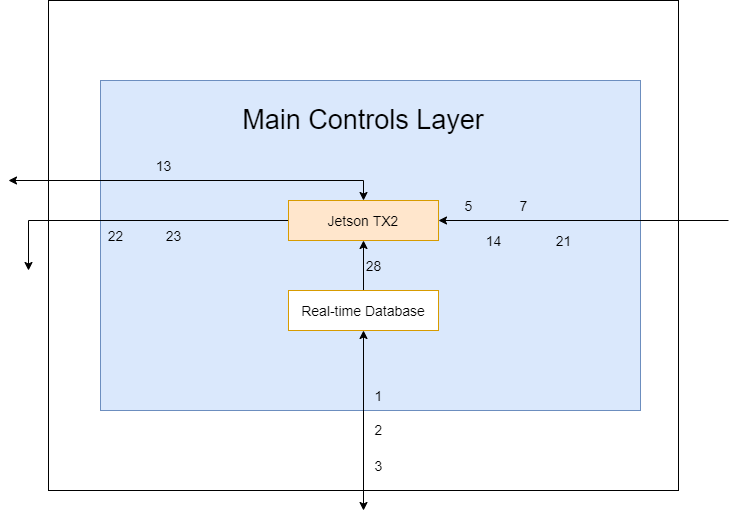
\includegraphics[width=0.60\textwidth]{images/Jetson.png}
 \caption{NVIDIA Jetson TX2 in the Main Controls Layer}
\end{figure}

\subsubsection{Assumptions}
It is assumed that the Jetson TX2 will be connected to WiFi the entire time it is active. 

\subsubsection{Responsibilities}
The Jestson TX2 will take in all inputs from the remote control, computer vision and other peripherals. With this data, it will be responsible for sending the appropriate signals to the corresponding peripherals.

\subsubsection{Subsystem Interfaces}
Each of the inputs and outputs for the subsystem are defined here.

\begin {table}[H]
\caption {Controls Software Interfaces} 
\begin{center}
    \begin{tabular}{ | p{1cm} | p{5cm} | p{3cm} | p{5cm} |}
    \hline
    ID & Description & Inputs & Outputs \\ \hline
    \#5 & Computer Vision Data & \pbox{3cm}{\phantom{Boo!}\\Optimized distance of target object(s) from camera\\ \\True position of target object(s) in 2D space\\} & \pbox{5cm}{N/A}  \\ \hline
    \#7 & Power & \pbox{3cm}{Power} & \pbox{5cm}{N/A}  \\ \hline
    \#13 & CAN Bus to Jetson & \pbox{3cm}{Motor RPM} & \pbox{3cm}{Desired Speed}   \\ \hline
    \#14 & Connection to the Microcontroller & \pbox{3cm}{Turing mechanism angle \\ Solenoid state} & \pbox{5cm}{Degrees to rotate turning mechanism \\ Toggle turning mechanism (on/off) \\ Toggle solenoid}  \\ \hline
    \#21 & Connection to Weight Sensor & \pbox{3cm}{\phantom{Boo!}\\Current weight value on board\phantom{Boo!}\\} & \pbox{5cm}{N/A}  \\ \hline
    \#22 & Connection to LEDs & \pbox{3cm}{N/A} & \pbox{5cm}{Mode Indicator Signal}  \\ \hline
    \#23 & Connection to Buzzer/Speaker & \pbox{3cm}{N/A} & \pbox{5cm}{Alert Signal}  \\ \hline
    \#28 & Data Fetching & \pbox{3cm}{\phantom{Boo!}\\User entered values\phantom{Boo!}\\} & \pbox{5cm}{}  \\ \hline
    \end{tabular}
\end{center}
\end{table}

\subsection{Real-Time Database}
The Turing Board's real-time database is will be hosted by Google Firebase. It will hold our data values per user and allow for a quick transfer of information over internet between the Turning Board's computing components.

\begin{figure}[h!]
	\centering
 	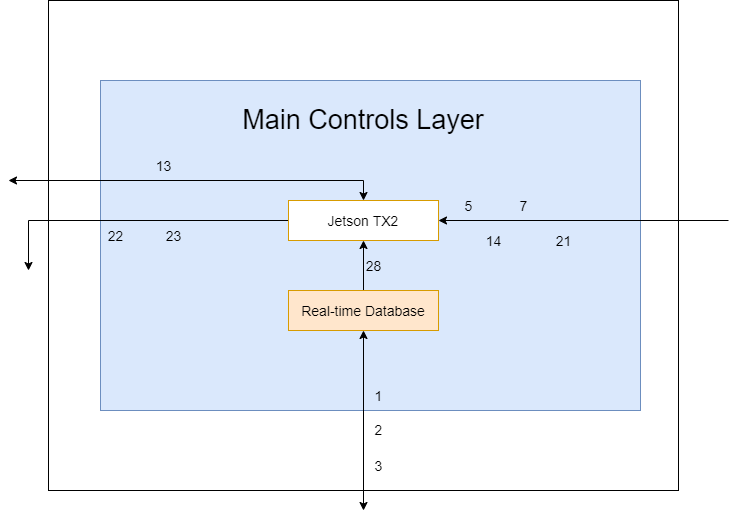
\includegraphics[width=0.60\textwidth]{images/RTD.png}
 \caption{The Real-Time Database in the Main Controls Layer}
\end{figure}

\subsubsection{Assumptions}
It is assumed that the Jetson TX2 and the user's phone (the remote control) will be connected to the internet the entire time it is active. This will allow for communication via the real-time database. 

\subsubsection{Responsibilities}
The real-time database will be responsible for storing user entered values from the remote control so the Jetson can compare those values with the current peripheral in order to make adjustment accordingly.

\subsubsection{Subsystem Interfaces}
Each of the inputs and outputs for the subsystem are defined here.

\begin {table}[H]
\caption {Controls Software Interfaces} 
\begin{center}
    \begin{tabular}{ | p{1cm} | p{5cm} | p{3cm} | p{5cm} |}
    \hline
    ID & Description & Inputs & Outputs \\ \hline
    \#1 & Front-end & \pbox{3cm}{Data from database to dispaly per screen on app} & \pbox{5cm}{User command}  \\ \hline
    \#2 & Authentication & \pbox{3cm}{Token} & \pbox{5cm}{User information}  \\ \hline
    \#3 & Ride analysis & \pbox{3cm}{\phantom{Boo!}\\legible ride analysis data\phantom{Boo!}\\} & \pbox{3cm}{refined database data}   \\ \hline
    \#28 & Data Fetching & \pbox{3cm}{N/A} & \pbox{5cm}{User entered values}  \\ \hline
    \end{tabular}
\end{center}
\end{table}